\newcommand{\templatesdir}{../../../templates}
\newcommand{\template}{template-roteiro-est}
\input{\templatesdir/\template/template}

\newcommand{\content}{Outras estruturas de dados lineares}
\newcommand{\class}{Algoritmos e Estruturas de Dados}
\newcommand{\shortcourse}{45EST}

\begin{document}

\makeheader

Leitura obrigatória:
\begin{itemize}
	\item Capítulo 10 de~\cite{DeitelAndDeitel2010} -- Coleções.
\end{itemize}

Leitura complementar:
\begin{itemize}
	\item Capítulo 12 de~\cite{Preiss2001} -- Conjuntos, multiconjuntos e partições.
\end{itemize}

\medskip

\newtitle{Java Collections}

\begin{itemize}
	\item O framework \texttt{java.util.Collections} fornece implementação para muitas estruturas de dados.
\end{itemize}

\begin{figure}[H]
	\centering
	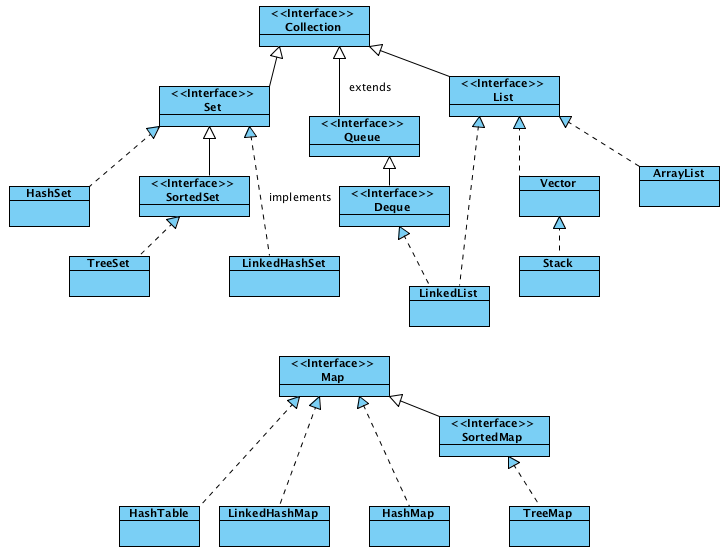
\includegraphics[width=0.74\linewidth]{img/collections}
\end{figure}

\clearpage

\textbf{Exemplos}

\begin{table}[H]
	\centering
	\begin{tabular}{lll}
		\hline
		\textbf{Estrutura} & \textbf{Interface} & \textbf{Implementações} \\
		\hline
		Pilha & \texttt{List} & \texttt{Stack} \\
		Fila & \texttt{Queue} & \texttt{LinkedList} \\
		Deque & \texttt{Deque} & \texttt{ArrayDeque}, \texttt{LinkedList} \\
		Lista dinâmica & \texttt{List} & \texttt{ArrayList}, \texttt{LinkedList} \\
		Fila de prioridade & \texttt{Queue} & \texttt{PriorityQueue} \\
		Mapa & \texttt{Map} & \texttt{HashTable}, \texttt{TreeMap} \\
		\hline
	\end{tabular}
\end{table}

\bigskip

\newtitle{Outras estruturas de dados}

\textbf{Tabelas hash}
\begin{itemize}
	\item Outra (e mais eficiente) forma de implementar um mapa.
	\item Também chamado de tabela de dispersão ou tabela de espalhamento.
	\item Utiliza uma \textit{função hash} que mapeia chaves para posições no vetor.
	\item A função calcula a posição que o elemento será/está armazenado.
	\item Operações básicas em tempo constante $O(1)$.
	\item \textbf{Implementação:} \texttt{Map}, \texttt{Hashtable}, \texttt{LinkedHashMap}, \texttt{HashMap}.
	\item \textbf{Operações:} \texttt{put}, \texttt{get}, \texttt{containsKey}, \texttt{remove}.
\end{itemize}

\clearpage

\textbf{Conjuntos}
\begin{itemize}
	\item Estrutura que armazena elementos sem repetição.
	\item Permite operações realizadas sobre conjuntos.
	\item \textbf{Implementação:} \texttt{Set}, \texttt{SortedSet}, \texttt{HashSet}.
	\item \textbf{Operações:} \texttt{add}, \texttt{contains}, \texttt{remove}, \texttt{addAll}, \texttt{removeAll}, \texttt{retainAll}.
\end{itemize}

\bigskip

\textbf{Multiconjuntos}
\begin{itemize}
	\item Trata-se de um conjunto que permite repetição de elementos.
	\item Também conhecido como \textit{bag}.
	\item A ordem é irrelevante: \texttt{\{a, b, c\} = \{b, c, a\}}.
	\item \textbf{Implementação:} utiliza-se um \texttt{ArrayList<E>} ou um \texttt{Map<E, Integer>} (contando os elementos).
	\item \textbf{Operações:} iguais às dos conjuntos.
\end{itemize}

\bigskip

\textbf{Multimapas}
\begin{itemize}
	\item Trata-se de um mapa que armazena múltiplos valores para uma mesma chave.
	\item \textbf{Implementação:} um mapa que permite repetição de chave, ou um mapa cuja entrada armazena a chave e uma lista de valores.
	\item \textbf{Operações:} iguais às dos mapas.
\end{itemize}

\clearpage

\newtitle{Classe Arrays}

\begin{itemize}
	\item A classe \texttt{java.util.Arrays} fornece implementação de vários métodos úteis no tratamento de coleções.
\end{itemize}

\begin{table}[H]
	\centering
	\begin{tabular}{ll}
		\hline
		\textbf{Método} & \textbf{Descrição} \\
		\hline
		\texttt{asList} & dado um vetor, devolve uma lista encadeada. \\
		\texttt{binarySearch} & executa uma busca binária na coleção recebida. \\
		\texttt{copyOf} & retorna uma cópia da coleção recebida. \\
		\texttt{equals} & compara se duas estruturas são iguais. \\
		\texttt{fill} & preenche a coleção pelo valor recebido. \\
		\texttt{sort} & ordena a coleção recebida. \\
		\texttt{toString} & devolve uma String com os elementos da coleção. \\
		\hline
	\end{tabular}
\end{table}

\medskip

\newtitle{Atividades}

\begin{enumerate}
	\item Refaça os exercícios de implementação utilizando as estruturas fornecidas pelo framework \texttt{java.util.Collections}.
	
	\item Desenvolva um programa para armazenar dados utilizando tabelas hash, conjuntos, multiconjuntos e multimapas. Explore as operações fornecidas pelo framework para essas estruturas de dados.
	
	\item Desenvolva um software que armazene produtos em um \texttt{ArrayList}. Utilize os métodos utilitários da classe \texttt{java.util.Arrays} para manipulação dessa estrutura.
\end{enumerate}

\clearpage

\newtitle{Referências}
\begingroup
	\footnotesize
	\renewcommand{\chapter}[2]{}%
	\bibliographystyle{apalike}
	\bibliography{../referencias}
\endgroup

\end{document}